
\section{Web Search}

\begin{breakbox}
\boxtitle{Evaluating IR System:}
\begin{itemize}
	\item Note: the information need is translated into a query.
	\item Query: wine red white heart attack effective.
	\item Relevance is assessed relative to the information need not the query.
	\item E.g., Information need: I'm looking for information on whether drinking red wine is more effective at reducing your risk of heart attacks than white wine.
	\item You evaluate whether the doc addresses the information need, not whether it has these words.
\end{itemize}
\end{breakbox}

\begin{breakbox}
\boxtitle{Precision \& Recall:}
\newline Confusion Matrix:
\begin{center}
\begin{tabular}{| l | l | l |}
\hline
 & Relevant & Nonrelevant \\ \hline
Retrieved	& True pos. (tp) & False pos. (fp) \\ \hline
Not Retrieved & False neg. (fn) & True neg. (tn) \\
\hline
\end{tabular}
\end{center}
\begin{itemize}
	\item Precision $= \frac{tp}{(tp + fp)} = \frac{\text{\# (found and relevant)}}{\text{\# found}}$
	\item Recall $= \frac{tp}{(tp + fn)} = \frac{\text{\# (found and relevant)}}{\text{\# relevant}}$
\end{itemize}
\begin{center}
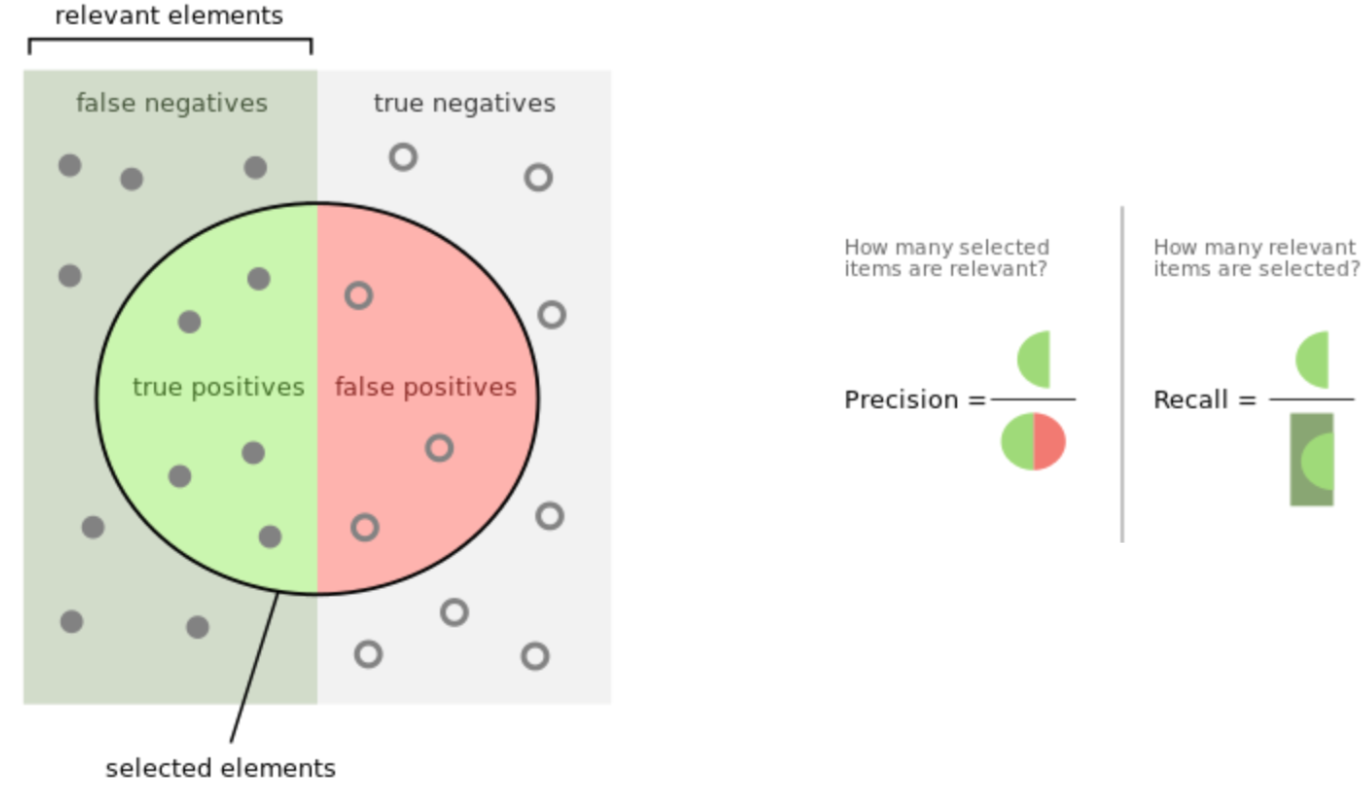
\includegraphics[width=.15\textwidth]{slides_images/precision_recall}
\end{center}
\end{breakbox}

\begin{breakbox}
\boxtitle{Notes:}
\begin{itemize}
	\item You can get high recall (but low precision) by retrieving all docs for all queries!
	\item Recall is a non-decreasing function of the number of docs retrieved
	\item In a good system, precision decreases as either the number of docs retrieved or recall increases.
\end{itemize}
\end{breakbox}

\begin{breakbox}
\boxtitle{Difficulties With Recall:}
\begin{itemize}
	\item Relevant docs. in doc. pool and relevant retrieved docs. From query: impossible!
	\item Should average over large document collection/query ensembles.
	\item Need human relevance assessments.
	\item Assessments have to be binary.
	\item Heavily skewed by collection/authorship.
	\item It is nearly impossible to calculate recall for web.
\end{itemize}
\end{breakbox}

\begin{breakbox}
\boxtitle{Precision/Recall Curve:}
\begin{center}
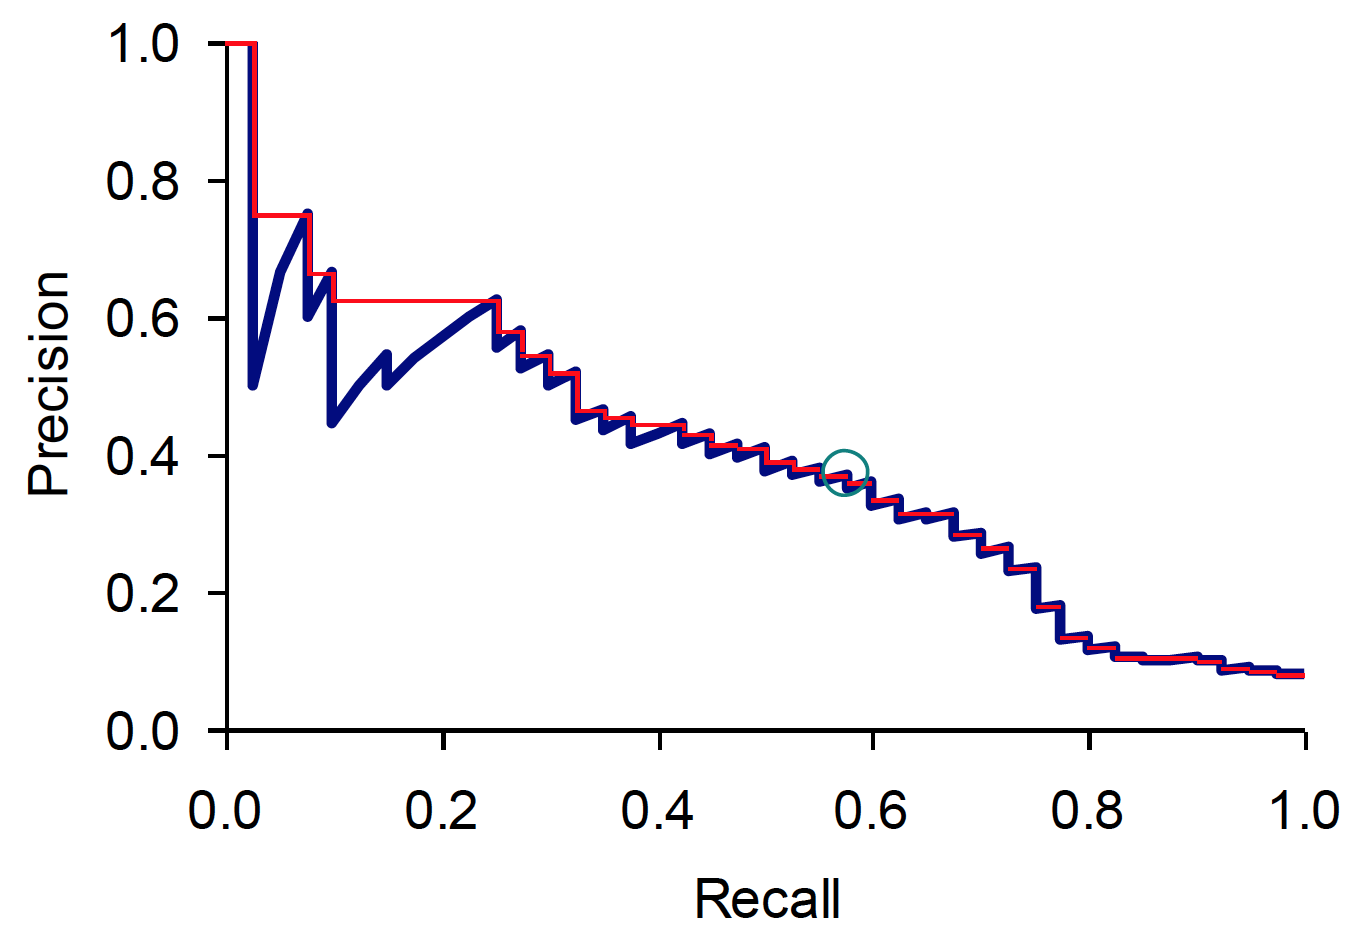
\includegraphics[width=.1\textwidth]{slides_images/precision_recall_curve}
\end{center}
\end{breakbox}

\begin{breakbox}
\boxtitle{A/B Testing:}
\begin{itemize}
	\item Purpose: Test a single innovation.
	\item Prerequisite: You have a large search engine up and running.
	\item Have most users continue to use the old system.
	\item Divert a small proportion of traffic (e.g., 1\%) to the new system that includes the innovation.
	\item Evaluate with an automatic measure like clickthrough-rate on first result.
	\item Now we can directly compare if the innovation does improve user happiness.
	\item Probably the evaluation methodology that large search engines trust most (def. used by Google).
	\item In principle this is less powerful than doing a multivariate regression analysis, but easier to understand.
\end{itemize}
\end{breakbox}

\begin{breakbox}
\boxtitle{Serch Engine Types:}
\begin{itemize}
	\item General purpose, horizontal SE
	\item Specialized SE:
		\begin{itemize}
			\item Vertical SE (by region, by topic, etc.)
			\item Deep Web
		\end{itemize}
	\item Meta-Search engines
\end{itemize}
\end{breakbox}

\begin{breakbox}
\boxtitle{The Web Document Collection:}
\begin{itemize}
	\item No design/co-ordination.
	\item Distributed content creation, linking, democratization of publishing.
	\item Content includes truth, lies, obsolete information, contradictions...
	\item Unstructured (text, html, ...), semi-structured (XML, annotated photos), structured (Databases)...
	\item Scale much larger than previous text collections ... but corporate records are catching up.
	\item Content can be dynamically generated.
\end{itemize}
\end{breakbox}

\begin{breakbox}
\boxtitle{Random Walks:}
\begin{itemize}
	\item View Web as directed graph.
	\item Build random walk on this graph:
		\begin{itemize}
			\item Includes various jump rules back to visited sites.
			\item Converges to a stationary distribution (Must assume graph is finite and time to convergence not really known).
			\item Use the strong query”method to check coverage by search engine.
		\end{itemize}
	\item Advantages:
		\begin{itemize}
			\item Statistically clean method at least in theory!
			\item Could work even for infinite web (assuming convergence) under certain metrics.
		\end{itemize}
	\item Disadvantages:
		\begin{itemize}
			\item List of seeds is a problem.
			\item Practical approximation might not be valid.
			\item Non-uniform distribution (subject to link spamming).
		\end{itemize}
\end{itemize}
\end{breakbox}

\begin{breakbox}
\boxtitle{Teleporting:}
\begin{itemize}
	\item At a dead end, jump to a random web page.
	\item At any non-dead end, with probability, say, 10\%, jump to a random web page.
	\item With remaining probability (90\%), go out on a random link.
	\item Cannot get stuck locally.
	\item There is a long-term rate at which any page is visited.
\end{itemize}
\end{breakbox}

\begin{breakbox}
\boxtitle{Query-Independent ordering:}
\begin{itemize}
	\item Undirected popularity: Each page gets a score = the number of in-links plus the number of out-links.
	\item Directed popularity: Score of a page = number of its in-links.
\end{itemize}
\end{breakbox}

\begin{breakbox}
\boxtitle{Hyperlink-Induced Topic Search (HITS):}
\begin{itemize}
	\item In response to a query, instead of an ordered list of pages each meeting the query, find two sets of inter-related pages:
		\begin{itemize}
			\item Hub pages are good lists of links on a subject (a good hub page for a topic points to many authoritative pages for that topic).
			\item Authority pages occur recurrently on good hubs for the subject (A good authority page for a topic is pointed to by many good hubs for that topic).
		\end{itemize}
	\item Gets at a broader slice of common opinion.
\end{itemize}
\end{breakbox}

\begin{breakbox}
\boxtitle{Page Ranking Example:}

\end{breakbox}
















